\subsection{Global}

    O método de limiarização global é o mais simples de ser implementado, e basta ter um limiar $T$ para dividir os pixels em dois conjuntos, $f(x,y) >= T$ e $f(x, y) < T$, atribuindo 255 e 0 aos pixels respectivamente.

    Esse método nos dá imagens binárias as quais a qualidade visual e o efeito de limiarização depende muito do limiar $T$ escolhido. Um exemplo pode ser observado na imagem \ref{fig:global}

    \begin{figure}[ht]
        \centering
        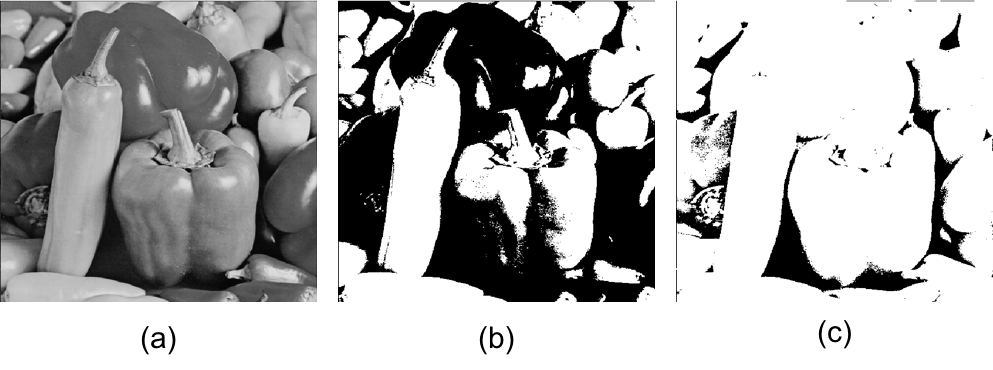
\includegraphics[width=\linewidth]{global.png}
        \caption{Imagens geradas através da aplicação do método de limiarização global para o \textit{peppers.png}. a, original. b limiarizada com $T=128$, c limiarizada com $T=50$.}
        \label{fig:gobal}
    \end{figure}

    De maneira geral, os resultados deste método não são muito bons se comparados aos demais estudados neste projeto.

\subsection{Bersen}

    No método de Bersen, para cada pixel $(x,y)$ da imagem, é calculado um limiar $T$ conforme a \ref{bersen}, onde $z_{min}$ e $z_{max}$ são os o mínimo e máximo local numa vizinhança de dimensão $n*n$ da imagem em relação ao pixel $(x,y)$.

    \begin{equation}
      T(x,y) = \dfrac{z_{min} + z_{max}}{2}
    \label{bersen}
    \end{equation}

    O resultado da aplicação deste método é uma imagem binária mas com um efeito interessante - surgem pontilhados nas áreas que tendem a ser homogêneas da imagem. Se for uma região escura, surgem pontos brancos e vice-versa.
    E quão maior for a vizinhança $n$ mais espaçados são esses pontilhados.
    Esse efeito pode ser observado na figura \ref{fig:bersen}.

    \begin{figure}[ht]
        \centering
        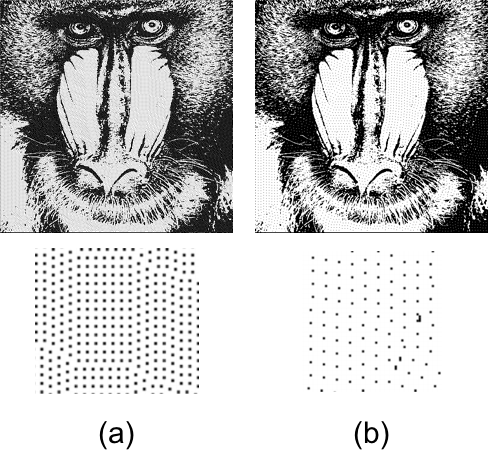
\includegraphics[width=\linewidth]{bersen.png}
        \caption{Imagens geradas através da aplicação do método de limiarização de Burkes para o \textit{baboon.png}, para $n = 4$ e $n = 10$, respectivamente a e b, com um corte em zoom da mesma área das duas imagens para comparação.}
        \label{fig:bersen}
    \end{figure}
